%************************************************
\chapter{The equatorial plane: The inner disk}\label{ch:ep} % $\mathbb{ZNR}$
%************************************************

Now that we understand the behavior of the geodesic movement along the axis of symmetry we will center our efforts in the movement restricted to the equatorial plane. The movement in the equatorial plane outside the horizons is well known in \gls{BL} coordinates. The fact that the metric is singular at the horizons prevent the geodesics to be extended across the horizons in this coordinate system. A complete analysis of the geodesic movement in the equatorial plane can be found in chapter 4 of \cite{o1995geometry}. The geodesic flow in the inner disk cannot be analyzed easily in \gls{BL} coordinates as the spacetime singularity is located at $r=0$ in this coordinates and therefore the ``ring`` shape cannot be analyzed in this coordinate system. The \gls{KS} coordinates are regular across all the horizons and in this system, the inner disk is well located at $x^2+y^2<a^2$ with $z=0$. Remember that this inner disk is the identification region between $\mathbb{R}_+$ and $\mathbb{R}_-$ as was previously noticed in \cref{ch:MAE}. As the geodesic behavior in the \gls{KS} coordinates in the equatorial plane is rather complicated and exceeds this work and because in the other hand, has been previously analyzed in more suitable coordinates, we are going to center our efforts in the inner disk.

\section{Hamiltonian equations of the geodesics}

We are going to discuss the geodesic equations inside the inner disk. Remember that this region is defined as $x^2+y^2<a^2$ with $z=0$. The complete understanding of the geodesic flow involves not only the knowledge of the geodesic equations but also the conditions that lead to future directed solutions. In this section we are going to derive the geodesic equations in the inner disk. 

\begin{theorem}\label{Th:ep}
 The geodesic equations for the Kerr metric restricted to the inner disk in \gls{KS} coordinates are the solution of the Hamilton equations derived from the Hamiltonian
 \begin{equation}
 H'=\frac{1}{2}  \vec{p}^{\,2}
\end{equation}
where $H=\frac{1}{2}(E^2-\mu)$ with $\mu=0$ for null geodesics, $\mu=1$ for timelike geodesics.
\end{theorem}
\begin{Proof}
Unless it is specified otherwise, $x^2+y^2<a^2$ is assumed. In the previous chapter, we derived a Hamiltonian ( see \cref{FinalgeneralH}) that describes the geodesic flow in the hole Kerr spacetime. We can adapt this Hamiltonian to the equatorial plane taking the limit $z \to 0$. This limit has to be computed carefully as we have terms involving $r(x,y,z)$ and $z$. The Hamiltonian is written as
\begin{equation}\label{Hamiltoniandisk}
H^{\prime}= \frac{1}{2}\left(E^2-\mu \right)
\frac{1}{2} \left( \vec{p}^{\,2}- \lim_{z \to 0}{(h)} \left( \vec{K} \cdot \vec{p} - E 
\hat{K} \right)^2 \right),
\end{equation} 
which is defined on the cotangent bundle of $\mathbb{R}^{3} \setminus \C$, where $\C$ represent the singular ring, $p=\left(p_x,p_y,0\right)$ $\vec{K}=\lim_{z \to 0}\left(\frac{x r(x,y,z)+a y}{r(x,y,z)^2+a^2},\frac{y r(x,y,z)-a x}{r(x,y,z)^2+a^2}, {\frac{z}{r(x,y,z)}}\right)$ and $\hat{K}=\sigma$. As we have studied before in \cref{ch:MAE}, the function $r(x,y,z)$ can be written near the inner disk as
 \begin{equation}
  r(x,y,z)=z \sqrt{f(x,y,\bar{z})},
 \end{equation}
 where $f(x,y,\bar{z})$ is a nonzero positive smooth function. Then, the limits can be written as
 \begin{align}
  &\lim_{z \to 0}{h}=  \lim_{z \to 0}{\frac{2 M r^3}{r^4+a^2 z^2}} =\lim_{z \to 0}{\frac{2 M (z \sqrt{f(x,y,\bar{z})})^3}{(z \sqrt{f(x,y,\bar{z})})^4+a^2 z^2}}\\
  &= \lim_{z \to 0}{\frac{2 M z f(x,y,\bar{z})^\frac{3}{2}}{ z^2 f(x,y,\bar{z})^2+a^2}}= 0,\\
  &\lim_{z \to 0}{h}=\frac{z}{r}=\frac{1}{\sqrt{f(x,y,\bar{z})}}
 \end{align}
The Hamiltonian becomes
\begin{equation}
 H'=\frac{1}{2}  \vec{p}^{\,2}
\end{equation}
so the solutions to the geodesic equations are
\begin{align}
 x(s)&=z_0 +{p_x}_0 s \\
 y(s)&=z_0 +{p_y}_0 s \\
 p_x(s)&={p_x}_0\\
 p_y(s)&={p_y}_0
\end{align}
where $s$ is the proper time $z(0)=z_0$ and $p_z(0)={p_z}_0$. With no difference if the geodesics are null or timelike.\end{Proof}

This result is very interesting because it tell us that the geodesic in the inner disk behaves as if the spacetime inside the singular ring were Minkowsky. This is analogous to the case in which a thin spherically symmetric shell is set as the source of the gravitational field. In this scenario and in virtue of Birkhoff's theorem \cite{birkhoff1923relativity} we will have the \gls{SW} metric outside the shell and the Minkowsky metric inside the shell. This also resembles the behavior of the electromagnetic field generated by a electrically charged thin shell, as in this case there is no field inside the shell and the field outside the shell behaves as the field generated by a punctual charge located at the center of the shell.

\section{Variation ranges and causal structure}\label{variationpe}
As we did in the previous chapter, we must now analyze the conditions that lead to future-oriented geodesics. This case is rather simple because the function $h_{z \to 0}=0$ for points inside the inner disk. 
\begin{lemma}
 If the time orientation of $(\M,g)$ is chosen so that
the null vector 
$K^\alpha=\left(-\sigma ,\frac{y}{a},-\frac{x}{a},\frac{\sqrt{a^2-x^2-y^2}}{a}\right)$
is future directed, then a geodesic with $\mu=0,1$ 
starting at a point $(t_0,x_0,y_0)$ with $x_0^2+y_0^2<a^2$ is future causal 
if and only if Carter's constant is positive for timelike geodesics and zero for null geodesics. 
\end{lemma}
\begin{Proof}
 As the function $h_{z \to 0}=0$ the metric in the inner disk becomes
 \begin{equation}
  g=\eta
 \end{equation}
 where $\eta$ is the Minkowsky metric. The 1-form $K$ of the Kerr metric becomes (after taking the limit $z \to 0$) $K=\left(-\sigma ,\frac{y}{a},-\frac{x}{a},\frac{\sqrt{a^2-x^2-y^2}}{a}\right)$ as $lim_{z \to 0} r(x,y,z)=0$ when $x^2+y^2<a^2$ and $\lim{z \to 0} \frac{z}{r(x,y,z)}=\frac{1}{\sqrt{f(x,y,\bar{z})}}=\frac{\sqrt{a^2-x^2-y^2}}{a}$. Before we can compute the conditions for future oriented geodesics notice that
 \begin{align}
  p_x&=dx(u)=\dot{x}, \label{eq:rel1} \\
  p_y&=dy(u)=\dot{y}, \label{eq:rel2} \\
  -E&=dt(u)=-\dot{t},\label{eq:rel3} \\
  L_z&= p_y x - p_x y= \dot{y} x- x \dot{y} \label{eq:rel4},
 \end{align}
 where $u=({t},\dot{x},\dot{y},0)$ is the tangent vector to the geodesics. The conditions that leads to future oriented casual (timelike and null) geodesics are $g(u_0, \sigma K |_{s=0}) <0$ or $g(u_0, \sigma K_{s=0}) =0$ which implies $u_0 = b \sigma K|_{s=0}$, with $b \geq 0$. This conditions reads
 \begin{equation}
  K_\alpha u^\alpha|_{s=0} = -a   \dot{t}_0+\sigma(\dot{y}_0 x_0-y_0 \dot{x}_0) \leq 0\\
 \end{equation}
where the equality is only when $u_0 = b \sigma K|_{s=0}$. There is still another relation that allows us to distinguish between null an timelike geodesics given by
 \begin{equation}
  -\mu = u_\alpha u^\alpha = -\dot{t}^2+\dot{x}^2+\dot{y}^2.
 \end{equation}
As $K^\alpha$ is a null vector, i.e $K^\alpha K_\alpha=0$, the condition $u_0 = b \sigma K|_{s=0}$ implies that $u_\alpha u^\alpha=\mu=0$. Using the \cref{eq:rel3,eq:rel4} we can rewrite this conditions as
\begin{align}
  &K_\alpha u^\alpha|_{s=0} \leq 0 \rightarrow -\sigma L_z+  a E = \mathcal{C}^{\frac{1}{2}} \geq 0\\
  &\frac{1}{2} \left( E^2-\mu \right) =  \frac{1}{2} \left( \dot{x}^2+\dot{y}^2 \right)
\end{align}
 where $C$ is the Carter's constant restricted to the equatorial plane that we have seen in \vref{Carterep} and the condition $\mathcal{C}^{\frac{1}{2}}=0$ occurs if
 $\mu=0$. Notice that the third equation is a direct consequence of \cref{Th:ep} because this equation can be written using \cref{eq:rel1,eq:rel2,Hamiltoniandisk} as
\begin{equation}
 \frac{1}{2}\left(E^2-\mu \right)=H^{\prime}=  \frac{1}{2} \left( \dot{x}^2+\dot{y}^2 \right)= \frac{1}{2} \vec{p}^{\,2}
\end{equation}
So, the only independent condition that lead to future casual geodesics is $\mathcal{C}>0$ ($\mu$=1) or $\mathcal{C}>0=0$ ($\mu=0$) as claimed.\end{Proof}

As we are going to see in the next section, causal geodesic with starting point at $x_0,y_0$ with $z_0=0$ and $x_0^2+y_0^2<a^2$ cannot remain in the inner disk.
\section{Stability of the inner disk}

Although the geodesic behavior of the inner disk is interesting, we are going to show that a geodesic that starts in the inner disk cannot remain in it. A heuristic argument that leads to this conclusion is that when we studied the axis of symmetry ($x=y=0$) the point $z=0$ was not a stable point, indeed, the geodesic flow go upwards the axis if $\dot{\bar{z}}_0=0$ (remember that $\bar z=\lambda z$, where $\lambda=\pm 1$). Now, we are going to extend this behavior to all geodesic that starts with $p_{\bar{z}}=0$ and $x_0^2+y_0^2<a^2$, $z=0$.
\begin{proposition}
 Only null geodesic that starts starts in the inner disk ($x_0^2+y_0^2<a^2$ and $\bar{z}=0$) with $\dot{\bar{z}}=0$ can remain in this region while timelike geodesics leaves the disk with $\ddot{\bar{z}}>0$.
\end{proposition}
\begin{Proof}Lets consider the general Hamiltonian that describes the geodesic flow in \gls{KS} coordinates along all the spacetime derived in \vref{Hamiltonkerrschild} that writes
\begin{equation}
H^{\prime} = \frac{1}{2} \left( \vec{p}^{\,2}- h \left( \vec{K} \cdot \vec{p} - E  \hat{K} \right)^2 \right),
\end{equation} 
defined on the cotangent bundle of $\mathbb{R}^{3} \setminus \C$, where $\C$ represent the singular ring. Here $\hat{K}=\sigma$, $\vec{p}=(p_x,p_y,p_{\bar{z}})$ and $K=-\sigma dt + \frac{r(x dx+y dy)}{r^2+a^2} + \frac{a(x dy-y dx)}{r^2+a^2}+\frac{z dz}{r}$. The function $r(x,y,z)$ is defined for points near the inner disk as
\begin{equation}
 r(x,y,\bar{z})=\bar{z} \sqrt{f(x,y,\bar{z})}
\end{equation}
where $f(x,y,\bar{z})$ is a nonzero positive smooth function. Let's start by checking what value of $p_{\bar{z_0}}$ satisfies $\dot{\bar{z}}_0=0$. The Hamilton equation for $\dot{\bar{z}}$ evaluated at $t=0 \to \bar{z}_0=0$ implies that
\begin{equation}
\dot{\bar{z}}_0=\frac{\partial H}{\partial p_{\bar{z}}}|_{t=0 \to z=0}=p_{\bar{z_0}}.
\end{equation}
So $\dot{\bar{z}}_0=0 \rightarrow p_{\bar{z_0}}=0$. We need to calculate now $\ddot{\bar{z}}_0>0$. To achieve this we are going to calculate $\dot{\bar{z}}$ and derive this equation. Then, using the Hamilton equations for $\dot{p}_x$ , $\dot{p}_y$ and $\dot{p}_z$ we can obtain the equation for $\ddot{\bar{z}}$ as a function of $z$,$p_z$,$x$,$y$,$p_x$ y $p_y$. As we will need the derivatives of $f(x,y,\bar{z})$ we can compute these from the equation that defines $r(x,y,z)$ that is
\begin{equation}
r^2 |\vec{x}|^2=\bar{z}^2 |\vec{x}|^2+r^2 \left(x^2+y^2\right).
\end{equation}
After substituting $r= \bar{z} \sqrt{f(x,y,\bar{z})}$ and derive we can obtain
\begin{align}
 \partial_x f(x,y,\bar{z})&=-\frac{2 x f(x,y,\bar{z})}{-2 \bar{z}^2 f(x,y,\bar{z})-a^2+x^2+y^2+\bar{z}^2},\\
 \partial_y f(x,y,\bar{z})&=-\frac{2 y f(x,y,\bar{z})}{-2 \bar{z}^2 f(x,y,\bar{z})-a^2+x^2+y^2+\bar{z}^2},\\
  \partial_{\bar{z}} f(x,y,\bar{z})&=\frac{2 \bar{z} (f(x,y,\bar{z})-1) f(x,y,\bar{z})}{-2 \bar{z}^2 f(x,y,\bar{z})-a^2+x^2+y^2+\bar{z}^2}.
\end{align}
The Hamilton equation $\dot{\bar{z}}=\frac{\partial H}{\partial p_{\bar{z}}}$ reads
\begin{equation}\label{eqzeta}
\hspace{-0.1\textwidth}
 \dot{\bar{z}}=\left(p_{\bar{z}}-\frac{4 f(x,y,\bar{z}) {\bar{z}}^3 \left(\frac{p_x \left(a y+\sqrt{f(x,y,\bar{z})} x {\bar{z}}\right)}{a^2+f(x,y,\bar{z}) {\bar{z}}^2}+\frac{p_y \left(\sqrt{f(x,y,\bar{z})} y {\bar{z}}-a x\right)}{a^2+f(x,y,\bar{z}) {\bar{z}}^2}-E+\frac{p_{\bar{z}}}{\sqrt{f(x,y,\bar{z})}}\right)}{2 \left( a^2 {\bar{z}}^2+f(x,y,\bar{z})^2 {\bar{z}}^4 \right)}\right)
\end{equation}
The general form of the rest Hamilton equations is quite complicated and not very enlightening to display, and therefore we are going to display the final result. After computing $\ddot{\bar{z}}$ by deriving \cref{eqzeta}, substituting the Hamilton equation for $\dot{p}_x$ , $\dot{p}_y$ and $\dot{p}_z$, and evaluating the result at $t=0$ (which implies that $x=x_0$, $y=y_0$ ,$\bar{z}=0$, $p_x=p_{x_0}$, $p_y=p_{y_0}$,$p_{\bar{z}}=0$) we obtain that
\begin{align}
 \ddot{x}_0&=0\\
  \ddot{y}_0&=0\\
   \ddot{\bar{z}}_0&=\frac{f(x,y,\bar{z})^{3/2} (a E-\sigma L_z)^2}{a^4}=\frac{f(x,y,\bar{z})^{3/2} \mathcal{C}}{a^4}\\
\end{align}
As from \cref{variationpe} timelike geodesics starting at the inner disk must have $\mathcal{C}>0$ and therefore $\ddot{\bar{z}}_0>0$ while null geodesics can have  $\mathcal{C}=0$ and remain in the inner disk as claimed.\end{Proof}
\begin{figure}[hpt!]
\begin{center}
 \centerline{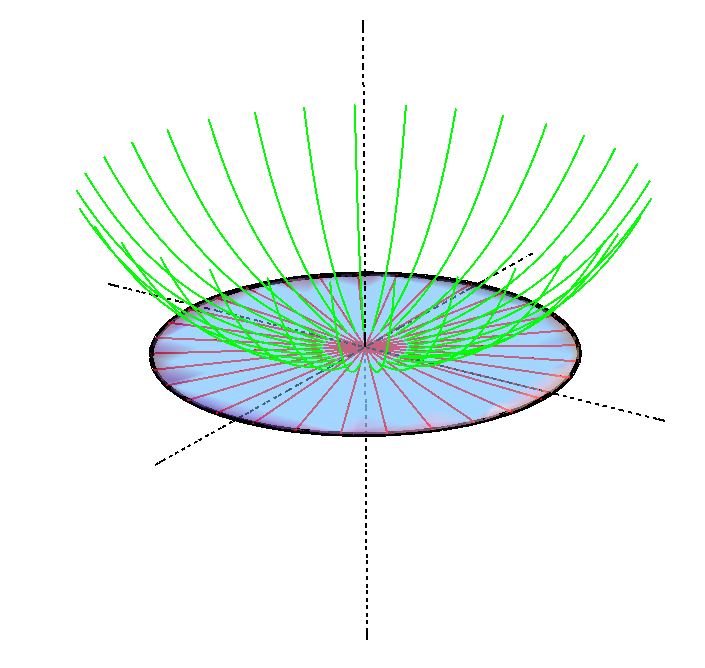
\includegraphics[width=0.75\textwidth]{img/Chapter5/Esc.png}}
 \end{center}
 \caption{The behavior of causal geodesics that start in the inner disk is depicted in this figure. The black dashed lines are the Cartesian axes, the green curves represent the causal geodesic at its first order of approximation, the red curves represent the background geodesic in the inner disk (the behavior that the geodesic would have if $\mathcal{C}=0$). The blue region represent the inner disk and the black ring represent the singular ring.}
 \label{fig:escape}
\end{figure} 

This shows that as the acceleration of the particle must be positive at the points in the inner disk, then the particle will start moving upwards $\bar{z}$ as is shows in \cref{fig:escape}. Of course, this is in perfect agreement with the results derived in \cref{ch:dinamicsys}, implying that a particle starting in $\bar{z}=0$ with $\dot{\bar{z}}=0$ will move in the direction that $\bar{z}$ increases (what we have called \textit{upwards}).

\section{A glimpse at the geodesics outside the inner disk}

As we said above, the geodesic flow outside the inner disk in the equatorial plane is hard to analyze, mostly because the causal structure is very complicated. In this section we are going to derive a energy-like equation for the geodesics in the Equatorial plane, that we are not going to analyze because it exceeds this work. The main difference between outside the ring and inside the ring is that outside the ring the function $r(x,y,z)$ is defined as
\begin{equation}\label{rinplane}
 \lim_{z \to 0} r(x,y,z)|_{x^2+y^2>a^2}= \sqrt{x^2+y^2-a^2}.
\end{equation}
and therefore the Hamiltonian \cref{Hamiltoniandisk} becomes in this case
\begin{equation}\label{Hamiltonplanoeq}
H^{\prime}= \frac{1}{2}\left(E^2-\mu \right)
\frac{1}{2} \left( \vec{p}^{\,2}- h \left( \vec{K} \cdot \vec{p} - E 
\hat{K} \right)^2 \right),
\end{equation} which is defined on the cotangent bundle of $\mathbb{R}^{3} \setminus \C$, where $\C$ represent the singular ring, $p=\left(p_x,p_y,0\right)$ $\vec{K}=\left(\frac{x r(x,y,z)+a y}{r(x,y,z)^2+a^2},\frac{y r(x,y,z)-a x}{r(x,y,z)^2+a^2},0\right)$ and $\hat{K}=\sigma$. The next theorem proofs that there exist a Energy-like equation for the geodesic movement in the equatorial plane.
\begin{theorem}
 The geodesic equations for the Kerr metric restricted to the equatorial plane outside the inner disk in \gls{KS} coordinates are the solution of the Energy-like equation
 \begin{equation}
 \frac{1}{2} \left( E^2-\mu \right) = \frac{1}{2} \left( \rho'^2 +\frac{L_z^2}{\rho^2}\right)-\frac{ M \mathcal{C}}{(\rho^2-a^2)^\frac{1}{2} \rho^2}-\frac{ \mu  M (\rho^2-a^2)^\frac{1}{2}}{\rho^2}.
 \end{equation}
where $\mathcal{C}$ is the Carter's constant, $L_z$ is the axial angular momentum, $\mu=1$ for timelike geodesics and $\mu=0$ for null geodesics and $\rho^2=r^2+a^2$.
\end{theorem}
\begin{Proof}
 The Hamiltonian \ref{Hamiltonplanoeq} reads
 \begin{equation}
  \frac{1}{2} \left( E^2-\mu \right)= H'=\frac{1}{2} \left(\vec{p}^{\,2}-\frac{h \left(E |\vec{x}|^2 +a (p_y x-p_x y)-r (p_x x+p_y y)\right)^2}{(|\vec{x}|^2)^2}\right)
 \end{equation}
 where $\vec{x}=(x,y)$. The angular momentum equation can be written from its definition ($L_z= p_y x - x p_y$) as $\vec{L_z}^2=(\vec{x} \times \vec{p})^2=\vec{x}^2 \vec{p}^{\,2}-(\vec{x} \cdot \vec{p})^2 $. We can use this relation to write the Hamiltonian as
 \begin{equation}\label{hamil2}
  H'=\frac{1}{2} \left(\frac{L_z^2+(\vec{x} \cdot \vec{p})^2}{|\vec{x}|^2}-\frac{h \left(E |\vec{x}|^2 +a L_z-r \vec{x} \cdot \vec{p}\right)^2}{|\vec{x}|^4}\right).
 \end{equation}
As from \cref{rinplane} one can derive that $r \dot{r} = \vec{x} \cdot \dot{\vec{x}}$, multiplying the Hamilton equation $\dot{\vec{x}}=\frac{\partial H}{\partial \vec{p}}$ by $\vec{x}$ we obtain that
\begin{equation}
 \vec{x} \cdot \dot{\vec{x}}=r \dot{r}=\frac{2 M \left(E |\vec{x}|^2 +a L_z\right)+\vec{x} \cdot \vec{p} (|\vec{x}|^2-2 M r)}{|\vec{x}|^2},
\end{equation}
from where we can solve for $\vec{x} \cdot \vec{p}$ and then, substituting this into the Hamiltonian of the \cref{hamil2}, which becomes
\begin{equation}
  H'= \frac{2 L_z^2 M |\vec{x}|^2+|\vec{x}|^2 \left(4 a E L_z M +2 E^2 M |\vec{x}|^2-L_z^2 r-r^3 r'^2\right)}{2 r |\vec{x}|^2 (2 M r-|\vec{x}|^2)}.
\end{equation}
As $H^{\prime}= \frac{1}{2}\left(E^2-\mu \right)$ we can write
\begin{equation}
\frac{1}{2}\left(E^2-\mu \right)=\frac{2 L_z^2 M |\vec{x}|^2+|\vec{x}|^2 \left(4 a E L_z M +2 E^2 M |\vec{x}|^2-L_z^2 r-r^3 r'^2 \right)}{2 r |\vec{x}|^2 (2 M r-|\vec{x}|^2)}.
\end{equation}
Rearranging this equation and substituting $|\vec{x}|^2=r^2+a^2$ can obtain
\begin{equation}
 E^2-\mu= r'^2+\frac{L_z^2}{r^2}-\frac{a^2 \left( E^2- \mu \right)}{r^2}-\frac{2 M \mathcal{C}}{r^3}-\frac{2 \mu  M}{r}
\end{equation}
which is not a Energy equation because it has $ E^2-\mu=2\epsilon$ (where $\epsilon$ is the Newtonian energy) in both sides. We can obtain get a new equation with the term $ E^2-\mu$ only in one side of the equation taking common factor in this term as
\begin{equation}
 \left( E^2-\mu  \right) \left( 1+\frac{a^2}{r^2} \right)= r'^2+\frac{L_z^2}{r^2}-\frac{2 M \mathcal{C}}{r^3}-\frac{2 \mu  M}{r}.
\end{equation}
Leaving alone this term in the left side the equation reads
\begin{equation}
 E^2-\mu =\left(\frac{r^2}{r^2+a^2} \right) r'^2 +\frac{L_z^2}{r^2+a^2}-\frac{2 M \mathcal{C}}{r(r^2+a^2)}-\frac{2 \mu  M r}{r^2+a^2}.
\end{equation}\label{preenergy}
which is not still a Energy-like equation because the term that goes with $ r'^2 $ is not a Kinetic-Energy term because it has the factor $\frac{r^2}{r^2+a^2} $. To finally obtain a Energy-like equation we can perform the transformation
\begin{equation}
 \rho^2=a^2+r^2
\end{equation}
as $\rho \rho ' = r r'$, then the \cref{preenergy} becomes
\begin{equation}
 \frac{1}{2} \left( E^2-\mu \right) = \frac{1}{2} \left( \rho'^2 +\frac{L_z^2}{\rho^2}\right)-\frac{ M \mathcal{C}}{(\rho^2-a^2)^\frac{1}{2} \rho^2}-\frac{ \mu  M (\rho^2-a^2)^\frac{1}{2}}{\rho^2}.
\end{equation}
\end{Proof}

First of all, notice that as the ring singularity is located at $x^2+y^2=r^2-a^2=a^2$ this implies that $r\in(0,\infty)$ and therefore $\rho \in (a,\infty)$. So the terms with $\rho^{-n}$ ($n>0$) are not divergence-terms because they are bounded by $\frac{1}{a^n} \leq \frac{1}{\rho^n}$. The true divergence-term is $(\rho^2-a^2)^{-\frac{1}{2}}$. We say that this is a Energy-like equation because it can be decomposed as
\begin{equation}
 \epsilon=\left( E^2-\mu \right) = T + V 
\end{equation}
where $T= \frac{1}{2} \left( \rho'^2 +\frac{L_z^2}{\rho^2}\right)$ is the kinetic energy in spherical-like coordinates and $V=V(\rho)=-\left( \frac{ M \mathcal{C}}{(\rho^2-a^2)^\frac{1}{2} \rho^2}+\frac{ \mu  M (\rho^2-a^2)^\frac{1}{2}}{\rho^2} \right)$ is the potential. Notice that as the Carter's constant depends on the Energy as $\mathcal{C}=(a E-\sigma L_z)^2$ this is not a true Energy equation, but can be analyzed like that if we impose this relation for the Carter's constant. Notice also that in the limit $a\to 0$ the equation becomes
\begin{equation}
 \frac{1}{2} \left( E^2-\mu \right) = \frac{1}{2} \left( \rho'^2 +\frac{L_z^2}{\rho^2}\right)-\frac{ M L_z^2}{\rho^3}-\frac{ \mu  M}{\rho}.
\end{equation}
that is the Energy equation for \gls{SW} geometry in \gls{KS} coordinates (see \cite{galindo2014mcgehee} for more information). To analyze the general Kerr Energy-like equation, we must obtain first the conditions that lead to future directed causal geodesics, but this task is quite complicated and exceeds the present work. As the ring singularity in some way regularizes the terms that diverge as $\frac{1}{\rho^n}$ (when we see the Kerr equation as an extension from the $\gls{SW}$ equation), we must deal only with the $(\rho^2-a^2)^{-\frac{1}{2}}$ divergence term. As was analyzed in \cite{galindo2014mcgehee}, once we have solved the conditions that lead to future directed casual geodesics, a interesting analysis of this equation would be based on apply the McGehee method to the phase space which derives from this equation. The Mcgehee method is a procedure that allows us to analyze the behavior of divergence dynamic systems near the singular points (and also \textit{in} the singular points). Although this is very interesting and novel, we left it for future work.
